\problemname{Closing Time}

Hungary is a country with $N$ cities, numbered from $0$ to
$N - 1$.

The cities are connected by $N - 1$ \emph{bidirectional} roads,
numbered from $0$ to $N - 2$. For each $j$ such that
$0 \le j \le N - 2$, road $j$ connects city $U[j]$ and city
$V[j]$ and has length $W[j]$, that is, it allows one to travel
between the cities in $W[j]$ units of time. Each road connects two
different cities, and each pair of cities is connected by at most one
road.

A \textbf{path} between two distinct cities $a$ and $b$ is a
sequence $p_0, p_1, \ldots, p_t$ of distinct cities, such that:
\begin{itemize}
  \item $p_0 = a$,
  \item $p_t = b$,
  \item for each $i$ ($0 \le i \leq t$), there
  is a road connecting cities $p_i$ and $p_{i + 1}$.
\end{itemize}
It is possible to travel from any city to any other city by using the
roads, that is, there exists a path between every two distinct cities.
It can be shown that this path is unique for each pair of distinct
cities.

The \textbf{length} of a path $p_0, p_1, \ldots, p_t$ is the sum of
the lengths of the $t$ roads connecting consecutive cities along the
path.

In Hungary, many people travel to attend the Foundation Day festivities
in two major cities. Once the celebrations are over, they return to
their homes. The government wants to prevent the crowd from disturbing
the locals, so they plan to lock down all cities at certain times. Each
city will be assigned a non-negative \textbf{closing time} by the
government. The government has decided that the sum of all closing times
must not be more than $K$. More precisely, for every $i$ between
$0$ and $N - 1$, inclusive, the closing time assigned to city $i$
is a nonnegative integer $c[i]$. The sum of all $c[i]$ must not be
greater than $K$.

Consider a city $a$ and some assignment of closing times. We say that
a city $b$ is \textbf{reachable} from city $a$ if and only if either
$b = a$, or the path $p_0, \ldots, p_t$ between these two cities (so
in particular $p_0 = a$ and $p_t = b$) satisfies the following
conditions:
\begin{itemize}
  \item the length of the path $p_0, p_1$ is at most $c[p_1]$, and
  \item the length of the path $p_0, p_1, p_2$ is at most $c[p_2]$, and
  \item $\ldots$
  \item the length of the path $p_0, p_1, p_2, \ldots, p_t$ is at most $c[p_t]$.
\end{itemize}

This year, the two main festival sites are located in city $X$ and
city $Y$. For each assignment of closing times, the
\textbf{convenience score} is defined as the sum of the following two
numbers:
\begin{itemize}
  \item The number of cities reachable from city $X$.
  \item The number of cities reachable from city $Y$.
\end{itemize}

Note that if a city is reachable from city $X$ and reachable from city
$Y$, it counts \emph{twice} towards the convenience score.

Your task is to compute the maximum convenience score that can be
achieved by some assignment of closing times.

\section*{Implementation Details}

You should implement the following procedure.

\begin{verbatim}
int max_score(int N, int X, int Y, int64 K, int[] U, int[] V, int[] W)
\end{verbatim}

\begin{itemize}
\item
  $N$: the number of cities.
\item
  $X$, $Y$: the cities with main festival sites.
\item
  $K$: the upper bound on the sum of closing times.
\item
  $U$, $V$: arrays of length $N - 1$ describing road connections.
\item
  $W$: array of length $N - 1$ describing road lengths.
\item
  This procedure should return the maximum convenience score that can be
  achieved by some assignment of closing times.
\item
  This procedure may be called \textbf{multiple times} in each test
  case.
\end{itemize}

\section*{Example}

Consider the following call:


\begin{center}
  \begin{tabular}{| l |}
    \hline
    \verb|max_score(7, 0, 2, 10,| \\
    \verb|[0, 0, 1, 2, 2, 5], [1, 3, 2, 4, 5, 6], [2, 3, 4, 2, 5, 3])| \\ \hline
  \end{tabular}
\end{center}


This corresponds to the following road network:

\begin{center}
  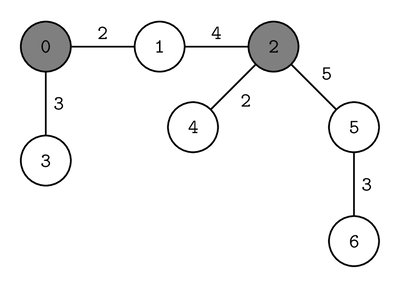
\includegraphics[scale=0.7]{0.png}
\end{center}

Suppose the closing times are assigned as follows:

\begin{center}
  \noindent
  \begin{tabular}[H!]{| l | l | l | l | l | l | l | l |}
    \hline
    \textbf{City} & $0$ & $1$ & $2$ & $3$ & $4$ & $5$ & $6$ \\ \hline
    \textbf{Closing time} & $0$ & $4$ & $0$ & $3$ & $2$ & $0$ & $0$ \\ \hline
  \end{tabular}
\end{center}

Note that the sum of all closing times is $9$, which is not more than
$K = 10$. Cities $0$, $1$, and $3$ are reachable from city $X$
($X = 0$), while cities $1$, $2$, and $4$ are reachable from
city $Y$ ($Y = 2$). Therefore, the convenience score is
$3 + 3 = 6$. There is no assignment of closing times with convenience
score more than $6$, so the procedure should return $6$.

Also consider the following call:

\begin{center}
  \begin{tabular}{| l |}
    \hline
    \verb|max_score(4, 0, 3, 20, [0, 1, 2], [1, 2, 3], [18, 1, 19])| \\ \hline
  \end{tabular}
\end{center}

\begin{verbatim}
\end{verbatim}

This corresponds to the following road network:

\begin{center}
  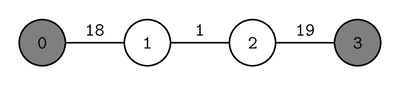
\includegraphics[scale=0.7]{1.png}
\end{center}

Suppose the closing times are assigned as follows:

\begin{center}
  \noindent
  \begin{tabular}[H!]{| l | l | l | l | l |}
    \hline
    \textbf{City} & $0$ & $1$ & $2$ & $3$ \\ \hline
    \textbf{Closing time} & $0$ & $1$ & $19$ & $0$ \\ \hline
  \end{tabular}
\end{center}


City $0$ is reachable from city $X$ ($X = 0$), while cities $2$
and $3$ are reachable from city $Y$ ($Y = 3$). Therefore, the
convenience score is $1 + 2 = 3$. There is no assignment of closing
times with convenience score more than $3$, so the procedure should
return $3$.

\section*{Constraints}

\begin{itemize}
\item
  $2 \le N \le 200\,000$
\item
  $0 \le X \leq Y \leq N$
\item
  $0 \le K \le 10^{18}$
\item
  $0 \le U[j] \leq V[j] \leq N$ (for each $j$ such that
  $0 \le j \le N - 2$)
\item
  $1 \le W[j] \le 10^6$ (for each $j$ such that
  $0 \le j \le N - 2$)
\item
  It is possible to travel from any city to any other city by using the
  roads.
\item
  $S_N \le 200\,000$, where $S_N$ is the sum of $N$ over all calls
  to \texttt{max\_score} in each test case.
\end{itemize}

\section*{Subtasks}

We say that a road network is \textbf{linear} if road $i$ connects
cities $i$ and $i + 1$ (for each $i$ such that
$0 \le i \le N - 2$).

\begin{enumerate}
\def\labelenumi{\arabic{enumi}.}
\item
  (8 points) The length of the path from city $X$ to city $Y$ is
  greater than $2K$.
\item
  (9 points) $S_N \le 50$, the road network is linear.
\item
  (12 points) $S_N \le 500$, the road network is linear.
\item
  (14 points) $S_N \le 3\,000$, the road network is linear.
\item
  (9 points) $S_N \le 20$
\item
  (11 points) $S_N \le 100$
\item
  (10 points) $S_N \le 500$
\item
  (10 points) $S_N \le 3\,000$
\item
  (17 points) No additional constraints.
\end{enumerate}

\section*{Sample Grader}

Let $C$ denote the number of scenarios, that is, the number of calls
to \texttt{max\_score}. The sample grader reads the input in the
following format:

\begin{itemize}
  \item line $1$: $C$
\end{itemize}

The descriptions of $C$ scenarios follow.

The sample grader reads the description of each scenario in the
following format:

\begin{itemize}
  \item line $1$: $N \; X \; Y \; K$
  \item line $2 + j$ ($0 \le j \le N - 2$): $U[j] \; V[j] \; W[j]$
\end{itemize}

The sample grader prints a single line for each scenario, in the
following format:

\begin{itemize}
  \item line $1$: the return value of \texttt{max\_score}
\end{itemize}
